% Simple poster (portrait)
% Author: Sofia Jijon (https://sjijon.github.io)
% Last Update: Sept 9, 2021
% Latest Version: https://github.com/sjijon/TeX-templates/tree/main/Tikzposter%20posters/Simple%20poster

\documentclass[a0paper,portrait,margin=0pt, colspace=24pt,subcolspace=0pt,blockverticalspace=36pt,innermargin=50pt]{tikzposter}

%\usepackage[latin9]{inputenc}
\usepackage[square,numbers]{natbib} 	    % Bibliography manager
\usepackage{amsmath,amssymb}
\usepackage{lipsum}  				        % Random Text
\usepackage[colalign]{aligncolsatbottom}    %To align columns at bottom (!! please run 2 times)

\usepackage{amsmath}                        %for the math!
\usepackage[utf8]{inputenc}                 %for the text


%***************%
%               %
%   Display     %
%               %
%***************%

\tikzposterlatexaffectionproofoff 			
\usetikzlibrary{shapes.geometric,arrows.meta,positioning}  %Tikz Libraries

% Fonts
\usepackage{helvet}					% Sans-Serif
\renewcommand{\familydefault}{\sfdefault}

% Colors
	\definecolor{MyOrange}{rgb}{0.8, 0.33, 0}
	\definecolor{MyBrown}{rgb}{0.28, 0.20, 0.20}
	\definecolor{MyGreen}{rgb}{0.33, 0.42, 0.18}

% Theme
\usetheme{Default}
\definecolorstyle{MyStyle2016}{
	\definecolor{ColorOne}{named}{MyBrown} 
	\definecolor{ColorTwo}{named}{MyOrange}
	\definecolor{ColorThree}{named}{MyGreen}
}{
    % Title Colors
    \colorlet{titlebgcolor}{ColorOne}
    \colorlet{titlefgcolor}{white}
    % Background Colors
    \colorlet{backgroundcolor}{ColorOne!15}
    \colorlet{framecolor}{ColorOne}
    % Block Colors
    \colorlet{blocktitlebgcolor}{white}
    \colorlet{blocktitlefgcolor}{ColorTwo}
    \colorlet{blockbodybgcolor}{white}
    \colorlet{blockbodyfgcolor}{black}
    % Innerblock Colors
    \colorlet{innerblocktitlebgcolor}{ColorOne!15}
    \colorlet{innerblocktitlefgcolor}{black}
    \colorlet{innerblockbodybgcolor}{ColorOne!15}
    \colorlet{innerblockbodyfgcolor}{black}
    % Note colors
    \colorlet{notebgcolor}{ColorTwo!20}
    \colorlet{notefgcolor}{ColorTwo}
    \colorlet{notefrcolor}{ColorTwo}
 }

% Color style
\usecolorstyle{MyStyle2016}

\title{Introduction to Algorithms and Data Structures}
\author{Zhivko Stoimchev}
\institute{	University of Primorska - Faculty of Mathematics, Natural Sciences and Information Technologies\\
	Koper, october 2022}


%***********%
%           %
%   BEGIN   %
%           %
%***********%

\begin{document}

%make title
\maketitle[width=0.96\linewidth,titletoblockverticalspace=36pt,linewidth=0,roundedcorners=10]

%MAKE COLUMNS!!
\begin{columns}


%***********%
%           %
%   LEFT    %
%           %
%***********%
\column{0.33}

%first block/field, with some text
\block[titleleft,roundedcorners=16]{Introduction to Alghorithms}{
	\par Algorithm is a step-by-step procedure, which defines a set of instructions to be executed in a certain order to get the desired output. Algorithms are generally created independent of underlying languages, i.e. an algorithm can be implemented in more than one programming language.
}

%second block/field with some text
\block[titleleft,roundedcorners=16]{Types of Algorithms}{
    \begin{itemize}
        \item Search - Algorithm to search an item in a data structure
        \item Sort - Algorithm to sort items in a certain order
        \item Insert - Algorithm to insert item in a data structure
        \item Update - Algorithm to update an existing item in a data structure
        \item Delete - Algorithm to delete an existing item from a data structure
    \end{itemize}
}

%third block/field with some text
\block[titleleft,roundedcorners=16]{Computer problems solved with Data Structures}{
    \begin{itemize}
    \item Fibonacci number series
    \item Knapsack problem
    \item Tower of Hanoi
    \item All pair shortest path by Floyd-Warshall
    \item Shortest path by Dijkstra
    \item Project scheduling
    \end{itemize}
}

%fourth block/field with some text and picture
\block[titleleft,roundedcorners=16]{Efficency Matters}{
	\par Different algorithms devised to solve the same problem often differ dramatically in their efficiency. These differences can be much more significant than differences due to hardware and software.
    
    %adding picture inside the block
    \begin{center}
		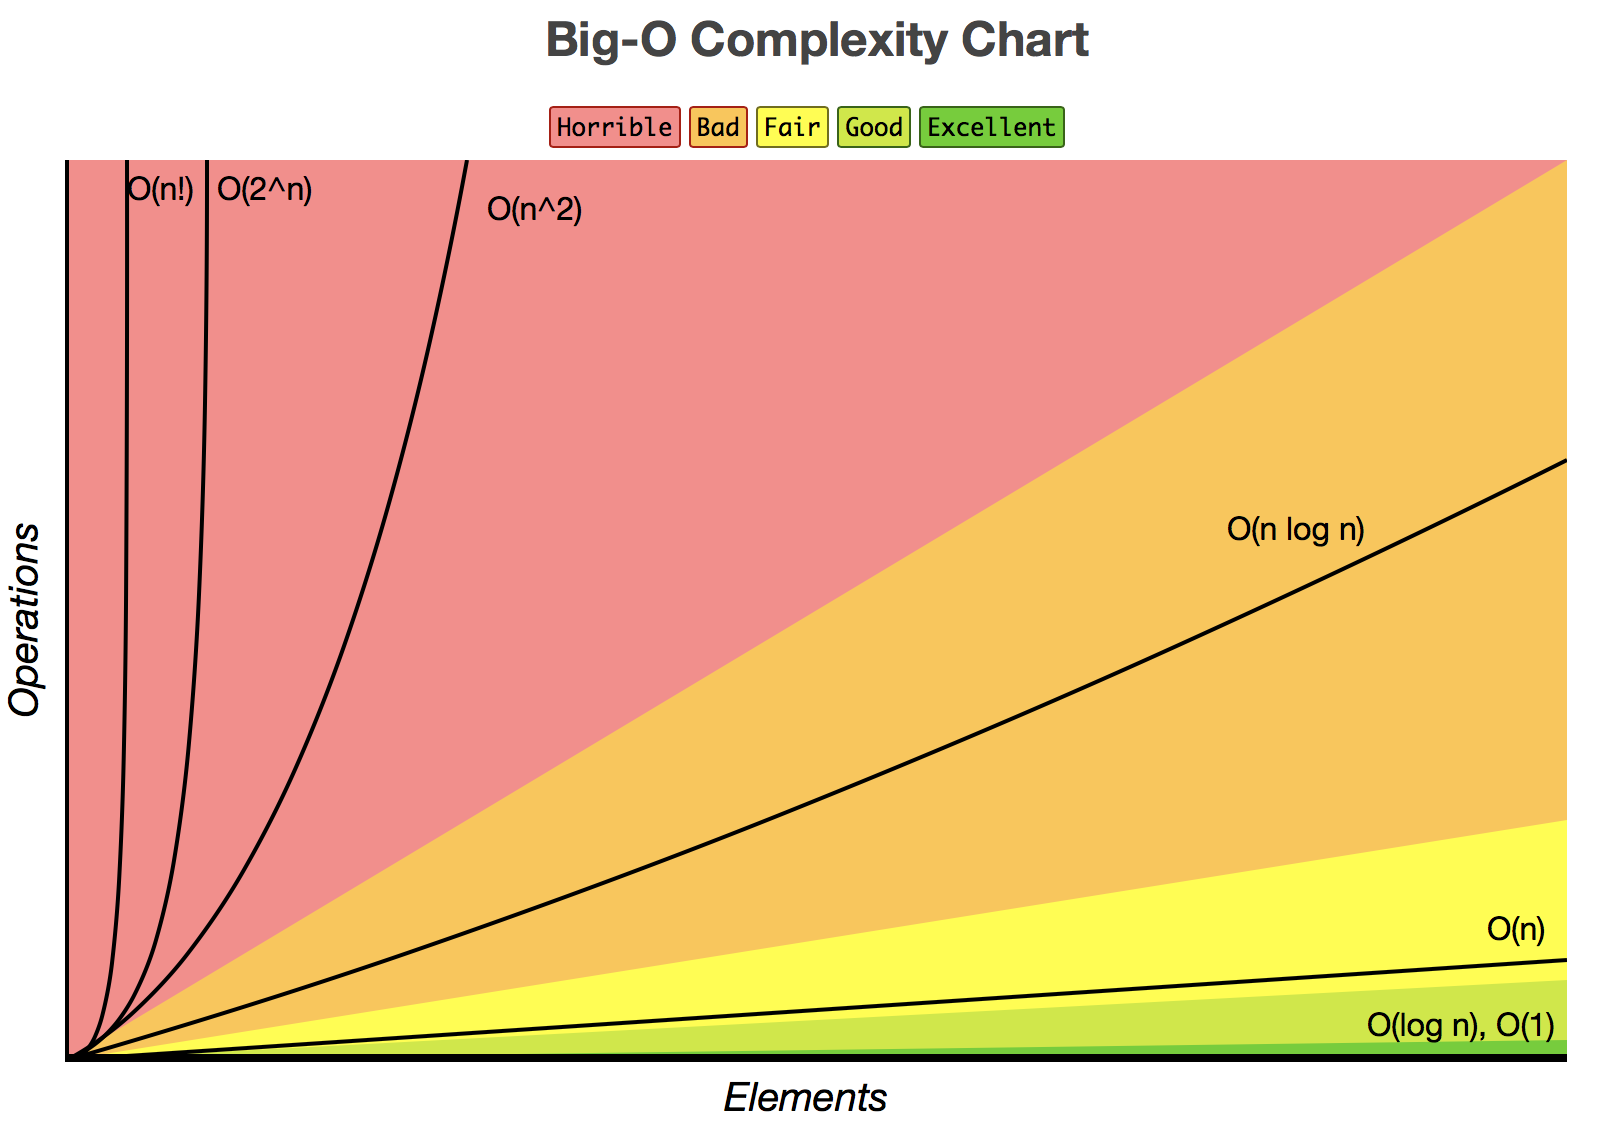
\includegraphics[width=1\linewidth]{img/alg eff cp.png}
	\end{center}
}


%***************%
%               %
%     MIDDLE    %
%               %
%***************%
\column{0.34}

%first block and introduction to algorithm complexity
\block[titleleft,roundedcorners=16]{Algorithm Complexity}{
	\par Suppose $X$ is an algorithm and n is the size of input data, the time and space used by the algorithm $X$ are the two main factors, which decide the efficiency of $X$.
	%add unordered list
	\begin{itemize}
	    \item Time Factor - Time is measured by counting the number of key operations such as comparisons in the sorting algorithm.
	    \item Space Factor - Space is measured by counting the maximum memory space required by the algorithm.
	\end{itemize}
}

%center image
\block[titleleft,roundedcorners=16]{ }{
    \begin{center}
        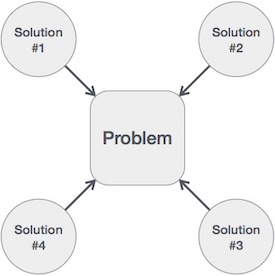
\includegraphics[width=1\linewidth]{img/problem.jpg}
    \end{center}
}

%second block explaining space complexity
\block[titleleft,roundedcorners=16]{Space Complexity}{
    \par Space complexity of an algorithm represents the amount of memory space required by the algorithm in its life cycle. The space required by an algorithm is equal to the sum of the following two components - 
    %add unordered list
    \begin{itemize}
        \item A fixed part that is a space required to store certain data and variables, that are independent of the size of the problem. For example, simple variables and constants used, program size, etc.
        \item A variable part is a space required by variables, whose size depends on the size of the problem. For example, dynamic memory allocation, recursion stack space, etc.
    \end{itemize}
 }
 
%third block explaining time complexity
\block[titleleft,roundedcorners=16]{Time Complexity}{
    Time complexity of an algorithm represents the amount of time required by the algorithm to run to completion. Time requirements can be defined as a numerical function $T(n)$, where $T(n)$ can be measured as the number of steps, provided each step consumes constant time.
    For example, addition of two $n$-bit integers takes $n$ steps. Consequently, the total computational time is $T(n) = c * n$, where $c$ is the time taken for the addition of two bits. Here, we observe that $T(n)$ grows linearly as the input size increases.
}


%************%
%            %
%   RIGHT    %
%            %
%************%
\column{0.33}

%first block explaining insertion sort
\block[titleleft,roundedcorners=16]{Visualising of Insertion Sort}{
    \par Insertion Sort is a sorting algorithm in which elements are taken from an unsorted item, inserting it in sorted order in front of the other items, and repeating until all items are in order. The algorithm is simple to implement and usually consists of two loops: an outer loop to pick items and an inner loop to iterate through the array. It works on the principle of the sorting playing cards in our hands. 

    %adding picture inside the block/ visualising insertion sort
    \begin{center}
		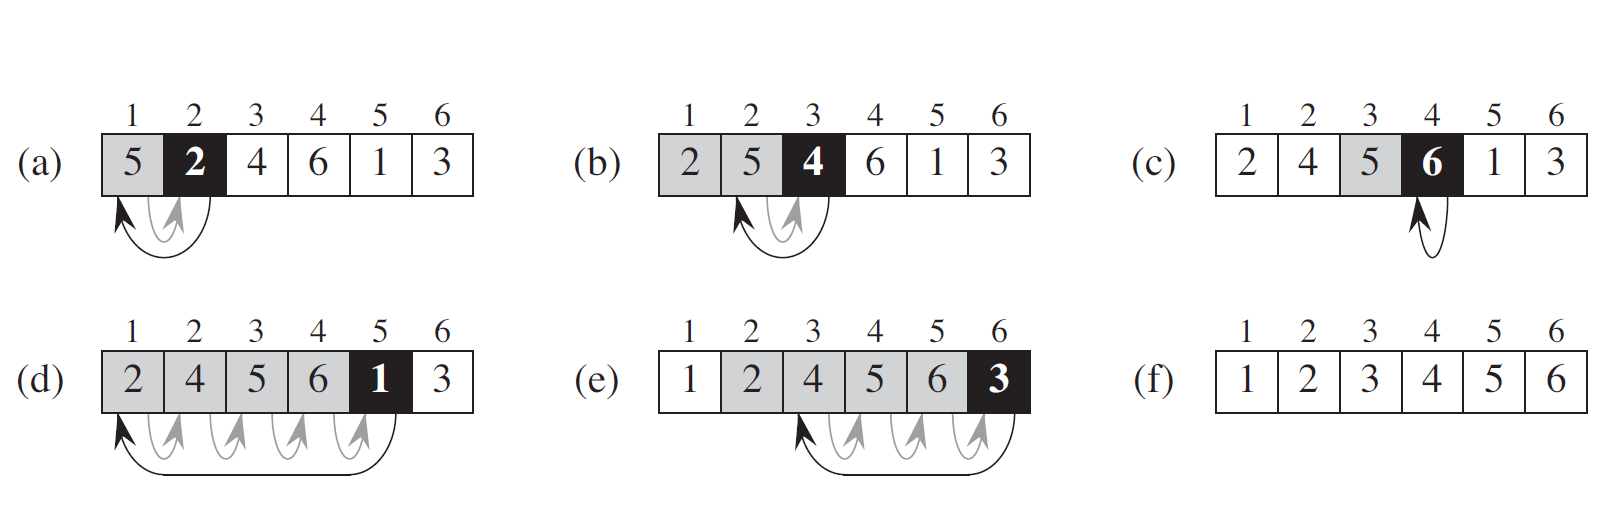
\includegraphics[width=1\linewidth]{img/insertion sort.png}
	\end{center}
	
	%add explanation to the picture
	\begin{center}
	    Complexity: $O(n^2)$
	\end{center}
 }
 
%second block visualising merge sort
\block[titleleft,roundedcorners=16]{Visualising Merge Sort}{
    \par Merge sort is an external algorithm based on the divide and conquer strategy. 
    \par Using the Divide and Conquer technique, the elements are split into two sub-arrays $(n/2)$ again and again until only one element is left, and then we sort the sub-arrays. 
    \par For this, merge sort uses three arrays, two of which are used to store each half, and the third one is uded to store the final sorted list by merging the other two.
    \par Bellow is a picture to helf visualizing the process:
    
    %add image
    \begin{center}
		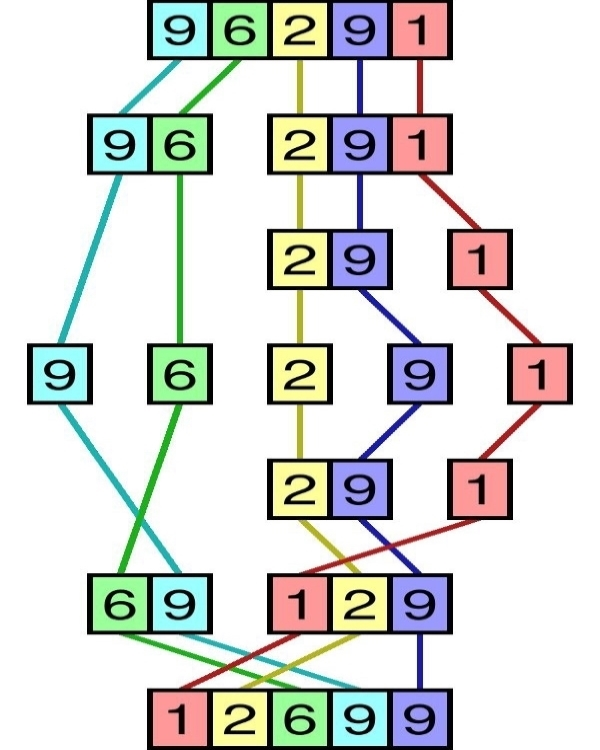
\includegraphics[width=1\linewidth]{img/merge cc.jpeg}
	\end{center}
	
	%add explanation to the picture
	\begin{center}
	    Complexity: $O(n logn)$
	\end{center}
}
 
%third block and conclusion
\block[titleleft,roundedcorners=16]{Conclusions}{
    \par We use algorithms in our everyday life, but we need to choose the one that fits the best and does the job the most efficiently. From the previous comparison between insertion sort and merge sort, we can conclude that merge sort is more efficient, and should use it whenever we can. It's not always the fastest way the best!
 }
 
\end{columns} 


%***********%
%           %
%   FOOT    %
%           %
%***********%

%references
\block[titleleft,roundedcorners=16]{}{
\small
\begin{minipage}{0.73\linewidth}
	\nocite{*}
	\bibliographystyle{unsrtnat}
	\bibliography{BibPoster}
 \end{minipage}
%
%	Logos
%
\begin{minipage}{0.2\linewidth}
\centering
	
\includegraphics[height=5cm]{img/famnit.png}
\end{minipage}
}
%
%	My info
%
\note[width=14.5cm,targetoffsetx=1cm,targetoffsety=3cm,rotate=15]{
	\textbf{Contact information:}\\
	Zhivko Zoran Stoimchev\\
	zivkostoimcev1551@outlook.com
}
\end{document}
